\documentclass[a0paper,fleqn]{betterposter}

%%%% Configuration (omitting most of the unused settings for brevity)

\renewcommand{\maincolumnbackgroundcolor}{theory}
\usepackage{caption}
\usepackage{natbib}
\begin{document}    
	\betterposter{
		%%%%%%%% SINGLE LEFT COLUMN (MERGED)
		
		\title{How do Bayesian Networks support impact-based forecasting for informed decision-making?}
		
		
		\section{Introduction}
		\begin{itemize}
			\item Impact-based forecasting (IBF) aims to support risk-oriented decisions in disaster risk management by promoting anticipatory actions that minimize damage and loss of life from natural hazards.
			\item A Bayesian Network (BN) is a directed graphical model representing a set of variables and their conditional probabilistic dependencies.
			\item IBF essentially uses risk matrices, which are products of the probability of impact and the extent of impact, represented as unconditional probabilities or impact numbers for events, like a flood event.
			\item However, it fails to consider conditional factors, potential interventions, and critical questions, such as the likelihood of significant consequences under different actions \citep{fenton2018risk}.
			
		\end{itemize}
		
		\section{Methods}
		\\ Method used for generating BN model, which can be extended with inputs and output applications for decision making.
		\begin{center}
		%\begin{figure}[h!]	
			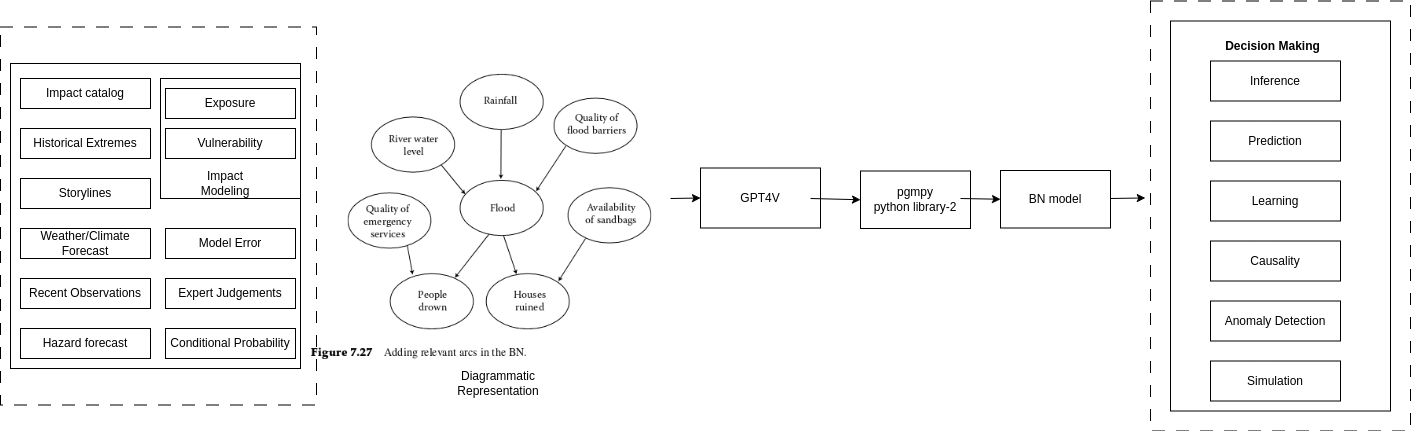
\includegraphics[width=\textwidth]{img/BN-model-IBF-v2.png}
			\captionof{figure}{\LARGE{BN generation steps, using GPTV4\citep{openai2023gpt4} and Python library pgmpy\citep{ankan2015pgmpy}, test image given is from \citep{fenton2018risk} }}
		%\end{figure}
		\end{center}
		
	    \section{Results}
		\begin{itemize}
			\item The Jupyter Notebook in Github shows the some of preliminary results related to the usage of simple Flood hazard anticipation and BN generation [4] 			
			\item Study is ongoing to extend the application
		\end{itemize}
		%% Institution logo
		%\includegraphics[width=\textwidth]{img/logo}\\
		\section{Reference}
		\begin{enumerate}
		\item 
		\item OpenAI. "GPT-4 Technical Report." arXiv e-prints, 2023, arXiv:2303.08774.
		%\item Ankan, Ankur, and Abinash Panda. 2015. [4]. 
		%\item Ankan, Ankur, and Abinash Panda. 2015. [4] \LARGE{"pgmpy: Probabilistic graphical models using python." Proceedings of the 14th python in science conference (scipy 2015). Vol. 10. Citeseer, 2015.}
		%\item \url{github.com/nishadhka/bn-ibf/code/01-simple-bn-flood.ipynb }
		\renewcommand{\bibsection}{}                                                                                                                                                                                                                                                                                                                                                                                                                                            
		\bibliographystyle{plainnat} % or another suitable style like abbrvnat, unsrtnat, etc.
		\bibliography{references} % if your file is named references.bib
		
		
	    \end{enumerate}
		\section{Authors: Nishadh K A, Viola Otieno, Jully Ouma, Collison Lorez, \& Ahmed Amdihun, ICPAC, Kenya}
		%\author{Mike Morrison}
		%\author{Rafael Bailo}
		%\institution{Optional Institution Under Name}
	}	
	{
		%%%%%%%% MAIN COLUMN
		\maincolumn{
			%%%% Main space
						
		Current \textbf{IBF} practices inadequately address \textbf{uncertainty, diverse perspectives, and process transparency}, leading to a lack of \textbf{'skin in the game'}. Integrating \textbf{Bayesian Networks} coupled with \textbf{GPT-4V/LLM} could revolutionize IBF.
			
		}{
			%%%% Bottom space
			\qrcode{img/qrcode-bn}{img/smartphoneWhite}{
				\textbf{Scan here} to proceed
				\\Github repo project
				\\nishadhka/bn-ibf
			}
		}
		
	}
	
\end{document}
